\chapter{Ondas guiadas e cavidades}\label{ch:b2:guided-waves}

O pulso de um radar vai do transmissor à antena parabólica dentro de um
tubo retangular de cobre; a luz de um enlace de internet viaja dez
mil quilômetros dentro de um fio de vidro mais fino que um cabelo; as
micro-ondas de um forno ricocheteiam entre suas paredes e se acomodam num
padrão de pontos quentes e frios. Uma onda confinada por paredes condutoras ou
refringentes deixa de ser uma onda plana livre para ir a qualquer lugar: ela
precisa satisfazer as condições de contorno nas paredes, e isso seleciona
as formas que ela pode tomar --- os \emph{modos} --- e a proíbe abaixo de uma
frequência de \emph{corte}. Este capítulo constrói o guia mais simples, duas
placas condutoras paralelas, a partir das reflexões do
\cref{ch:b2:wave-interfaces}; depois o \omterm{prop:b2:guided-waves:rectangular}{guia de ondas retangular}, a
cavidade fechada e, na imagem dos raios, a \omterm{prop:b2:guided-waves:fibre}{fibra óptica}.

\section{Ondas entre duas placas condutoras}

\begin{proposition}[Modos do guia de placas paralelas]\label{prop:b2:guided-waves:plates}
\index{guia de ondas}\index{onda guiada}\index{modo (guia de ondas)}\index{frequência de corte (guia de ondas)}
Dois planos perfeitamente condutores $y = 0$ e $y = a$ limitam o vácuo.
Procure uma onda que viaja segundo $z$ com $\vect E = E(y)\,\eu^{\iu(\omega t - k_gz)}
\vect e_x$ (o campo paralelo às placas, perpendicular à
propagação). As \omterm{thm:b2:maxwell-equations:maxwell}{equações de Maxwell} no vácuo e a condição $E = 0$
nas placas impõem
\[
E(y) = E_0\sin\frac{n\pi y}a , \qquad
k_g^2 = \frac{\omega^2}{c^2} - \Bigl(\frac{n\pi}a\Bigr)^2 , \qquad n = 1, 2, \dots
\]
O modo $n$ só se propaga acima de sua \emph{frequência de corte} $f_n = nc/2a$;
abaixo dela, $k_g$ é imaginário e o campo decai ao longo do guia. Suas
\omterm{def:b2:dispersion-wave-packets:relation}{velocidades de fase} e de grupo valem
\[
v_\varphi = \frac c{\sqrt{1 - f_n^2/f^2}} > c , \qquad
v_g = c\sqrt{1 - f_n^2/f^2} < c , \qquad v_\varphi v_g = c^2 ,
\]
e seu campo magnético tem componentes segundo $y$ e segundo $z$: uma
\omterm{prop:b2:guided-waves:plates}{onda guiada} não é transversal na direção de propagação.
\end{proposition}

\begin{proof}
Insira em $\Delta\vect E = \partial_t^2\vect E/c^2$: $E'' - k_g^2E = -(\omega^2/c^2)E$, ou seja,
$E'' + (\omega^2/c^2 - k_g^2)E = 0$, cujas soluções que se anulam em $y = 0$ e
$y = a$ são os senos com $\omega^2/c^2 - k_g^2 = (n\pi/a)^2$; $\operatorname{div}
\vect E = 0$ vale porque $E_x$ não depende de $x$. Faraday dá
$\underline B_y = (k_g/\omega)\underline E$ e $\underline B_z = (\iu/\omega)\partial_y\underline E$, este último
em quadratura. As velocidades seguem da forma de Klein--Gordon da
\omterm{def:b2:dispersion-wave-packets:relation}{relação de dispersão} (\cref{ch:b2:dispersion-wave-packets}).
\end{proof}

\begin{remark}[O modo como duas ondas planas]\label{rem:b2:guided-waves:zigzag}
$\sin(n\pi y/a)\eu^{-\iu k_gz}$ é a soma de duas ondas planas com
vetores de onda $(0, \pm n\pi/a, k_g)$, de módulo $\omega/c$, que ricocheteiam entre
as placas com o ângulo $\theta$ em relação ao eixo, com $\cos\theta = k_gc/\omega$:
um modo guiado é uma onda plana ziguezagueando entre as paredes, refletida
com $r = -1$ em cada uma, sendo a \omterm{prop:b2:waves-on-strings:modes}{onda estacionária} transversal a
condição de que ela interfira construtivamente consigo mesma. A energia
viaja ao longo do ziguezague a $c$, e portanto ao longo do eixo a $c\cos\theta = v_g$;
as interseções das cristas com o eixo correm a $c/\cos\theta = v_\varphi$. No
corte, a onda vai e volta atravessando o guia e não vai a
lugar algum.
\end{remark}

\begin{omfigure}
\begin{tikzpicture}[font=\small, x=1cm, y=1cm, >=Stealth]
  \begin{scope}
    \draw[thick] (-3,0) -- (3,0); \draw[thick] (-3,2) -- (3,2);
    \fill[pattern=north east lines] (-3,-0.15) rectangle (3,0); \fill[pattern=north east lines] (-3,2) rectangle (3,2.15);
    \draw[omDef, thick, ->] (-2.8,0.2) -- (-1.6,1.8); \draw[omDef, thick, ->] (-1.6,1.8) -- (-0.4,0.2); \draw[omDef, thick, ->] (-0.4,0.2) -- (0.8,1.8); \draw[omDef, thick, ->] (0.8,1.8) -- (2.0,0.2); \draw[omDef, thick, ->] (2.0,0.2) -- (2.8,1.27);
    \draw (-0.4,0.2) -- (0.6,0.2); \draw (0.3,0.2) arc[start angle=0, end angle=53, radius=0.7]; \node[font=\footnotesize] at (0.75,0.55) {$\theta$};
    \draw[->, thick] (-3,-0.6) -- (3,-0.6) node[right, font=\footnotesize] {$z$};
    \node[font=\footnotesize] at (-3.3,1) {$a$};
    \draw[<->] (-3.15,0) -- (-3.15,2);
  \end{scope}
  \begin{scope}[xshift=8.4cm]
    \draw[thick] (0,0) -- (0,2); \draw[thick] (3.6,0) -- (3.6,2);
    \fill[pattern=north east lines] (-0.15,0) rectangle (0,2); \fill[pattern=north east lines] (3.6,0) rectangle (3.75,2);
    \draw[omThm, thick, domain=0:3.6, samples=50] plot (\x,{1+0.8*sin(50*\x)});
    \draw[omProp, thick, domain=0:3.6, samples=50] plot (\x,{1+0.6*sin(100*\x)});
    \draw[dashed] (0,1) -- (3.6,1);
    \node[omThm, font=\footnotesize] at (1.8,2.3) {$n = 1$}; \node[omProp, font=\footnotesize] at (0.9,1.9) {$n = 2$};
    \draw[<->] (0,-0.3) -- (3.6,-0.3) node[midway, below, font=\footnotesize] {$a$ (o eixo $y$)};
  \end{scope}
\end{tikzpicture}

{\small À esquerda: um modo guiado é uma onda plana que ricocheteia entre as
placas; o ângulo $\theta$ se abre quando a frequência se aproxima do corte.
À direita: os perfis transversais $E(y)$ dos dois primeiros modos, que se anulam
nas paredes condutoras.}
\end{omfigure}

\begin{omfigure}
\begin{tikzpicture}
\begin{axis}[omaxis, axis x line=bottom, axis y line=left, width=6.6cm, height=4.8cm,
    xlabel={$k_g$}, ylabel={$\omega$}, xmin=0, xmax=3, ymin=0, ymax=4, xtick=\empty, ytick={1,2,3}, yticklabels={$\omega_1$, $\omega_2$, $\omega_3$}, samples=80,
    xlabel style={at={(axis description cs:1.0,0.0)}, anchor=west},
    ylabel style={at={(axis description cs:0.0,1.0)}, anchor=south}]
  \addplot[omThm, thick, domain=0:3] {sqrt(1+x*x)};
  \addplot[omThm, thick, domain=0:3] {sqrt(4+x*x)};
  \addplot[omThm, thick, domain=0:3] {sqrt(9+x*x)};
  \addplot[omDef, dashed, domain=0:3] {x};
  \node[font=\scriptsize, anchor=west] at (axis cs:2.2,2.05) {$\omega = ck_g$};
\end{axis}
\end{tikzpicture}
\hfill
\begin{tikzpicture}
\begin{axis}[omaxis, axis x line=bottom, axis y line=left, width=6.6cm, height=4.8cm,
    xlabel={$f/f_1$}, ylabel={$v/c$}, xmin=1, xmax=4, ymin=0, ymax=2.5, xtick={1,2,3,4}, ytick={1}, samples=100,
    xlabel style={at={(axis description cs:0.5,-0.12)}, anchor=north},
    ylabel style={at={(axis description cs:-0.1,0.5)}, rotate=90, anchor=south},
    legend style={font=\scriptsize, at={(0.97,0.95)}, anchor=north east, draw=none, fill=none}]
  \addplot[omThm, thick, domain=1.05:4] {1/sqrt(1-1/(x*x))};
  \addplot[omDef, thick, domain=1:4] {sqrt(1-1/(x*x))};
  \addplot[black, dashed, domain=1:4] {1};
  \legend{$v_\varphi$, $v_g$}
\end{axis}
\end{tikzpicture}

{\small À esquerda: as curvas de dispersão dos três primeiros modos de um
guia, cada uma uma hipérbole que começa em seu corte. À direita: as \omterm{def:b2:dispersion-wave-packets:relation}{velocidades de fase} e
de grupo de um modo em função da frequência; a energia rasteja perto do
corte e se aproxima de $c$ bem acima dele.}
\end{omfigure}

\begin{example}[Números]\label{ex:b2:guided-waves:numbers}
Placas a \qty{3}{cm} uma da outra: $f_1 = \qty{5}{GHz}$, $f_2 = \qty{10}{GHz}$; entre
essas frequências só um modo se propaga (operação \emph{monomodo},
que impede um pulso de se dividir em vários com
$v_g$ diferentes). A \qty{8}{GHz} o modo $n = 1$ tem $v_g = 0.78c$, $v_\varphi =
1.28c$, e o comprimento de onda no guia $\lambda_g = 2\pi/k_g = \qty{4.8}{cm}$, em vez dos
\qty{3.75}{cm} no espaço livre. A \qty{4}{GHz} nada passa: o campo
decai como $\eu^{-z/\ell}$ com $\ell = c/2\pi\sqrt{f_1^2 - f^2} = \qty{1.6}{cm}$ --- é o
princípio da tela na porta de um forno, do \omterm{prop:b2:guided-waves:plates}{guia de ondas} abaixo do corte
usado como atenuador calibrado, e dos dutos metálicos de
ventilação que deixam passar ar, mas não rádio.
\end{example}

\section{O guia de ondas retangular e a cavidade}

\begin{proposition}[O guia retangular; o modo TE$_{10}$]\label{prop:b2:guided-waves:rectangular}
\index{guia de ondas retangular}\index{modo TE}
Um tubo metálico oco de seção retangular $a \times b$ ($a > b$) carrega
modos cujas frequências de corte valem
\[
f_{mn} = \frac c2\sqrt{\Bigl(\frac ma\Bigr)^2 + \Bigl(\frac nb\Bigr)^2} ;
\]
o mais baixo, o \emph{\omterm{prop:b2:guided-waves:rectangular}{modo TE}$_{10}$} ($f_{10} = c/2a$), tem $\vect E = E_0\sin
(\pi x/a)\,\eu^{\iu(\omega t - k_gz)}\,\vect e_y$: meia senoide ao longo do lado
largo, uniforme ao longo do lado estreito, anulando-se nas duas paredes $x = 0$,
$x = a$ --- exatamente o modo das placas paralelas, sendo as paredes laterais $y = 0$, $b$
perpendiculares a $\vect E$ e nada lhe impondo. O guia é
usado entre $f_{10}$ e o corte seguinte; suas linhas de campo magnético
se fecham no plano $xz$, e as correntes que elas induzem nas paredes são
o que uma fenda não deve cortar. A potência transportada vale $\tfrac14\varepsilon_0cE_0^2\,ab
\sqrt{1 - f_{10}^2/f^2}$.
\end{proposition}

\begin{proof}
O modo geral é um produto de $\cos$ e $\sin$ em $x$ e $y$ com as
condições de contorno nas quatro paredes, o que dá $k_g^2 = \omega^2/c^2 - (m\pi/a)^2
- (n\pi/b)^2$ (admitido no caso geral; o caso TE$_{10}$ é a proposição
acima). Potência: o \omterm{thm:b2:poynting-vector:poynting}{vetor de Poynting} médio segundo $z$ vale $E_0^2\sin^2(\pi x/a)
\,k_g/2\mu_0\omega$, integrado na seção.
\end{proof}

\begin{omfigure}
\begin{tikzpicture}[font=\small, x=1cm, y=1cm, >=Stealth]
  \begin{scope}
    \draw[thick] (0,0) rectangle (3.6,1.8);
    \foreach \x in {0.45,0.9,...,3.15} {
      \pgfmathsetmacro{\h}{0.75*sin(deg(180*\x/3.6))}
      \draw[omDef, ->] (\x,{0.9-\h}) -- (\x,{0.9+\h});
    }
    \node[font=\footnotesize] at (1.8,-0.35) {$a$}; \node[font=\footnotesize] at (-0.3,0.9) {$b$};
    \node[omDef, font=\footnotesize] at (1.8,2.15) {TE$_{10}$: $\vect E$ ao longo do lado estreito};
  \end{scope}
  \begin{scope}[xshift=7.0cm]
    \draw[thick] (0,0) rectangle (4.8,1.8);
    \draw[omProp, thick, postaction={decorate, decoration={markings, mark=at position 0.2 with {\arrow{>}}, mark=at position 0.7 with {\arrow{>}}}}] (1.2,0.9) ellipse (0.9 and 0.55);
    \draw[omProp, thick, postaction={decorate, decoration={markings, mark=at position 0.2 with {\arrow{<}}, mark=at position 0.7 with {\arrow{<}}}}] (3.6,0.9) ellipse (0.9 and 0.55);
    \node[omProp, font=\footnotesize] at (2.4,2.15) {$\vect B$ em espiras no plano $xz$ (vista de cima)};
    \draw[->, thick] (0,-0.85) -- (1.2,-0.85) node[right, font=\footnotesize] {$z$};
    \draw[<->] (0,-0.3) -- (2.4,-0.3) node[midway, below, font=\footnotesize] {$\lambda_g/2$};
  \end{scope}
\end{tikzpicture}

{\small O \omterm{prop:b2:guided-waves:rectangular}{modo TE}$_{10}$ de um guia retangular: o campo elétrico
percorre a dimensão estreita com um perfil de meia senoide ao longo da
larga; o campo magnético se fecha em espiras no plano das faces
largas, com meio comprimento de onda de guia.}
\end{omfigure}

\begin{proposition}[Cavidade ressonante]\label{prop:b2:guided-waves:cavity}
\index{cavidade ressonante}\index{modo (cavidade)}
Fechar um guia com duas paredes condutoras separadas de um comprimento $d$ transforma-o
numa \emph{cavidade}, na qual a \omterm{prop:b2:guided-waves:plates}{onda guiada} precisa formar uma \omterm{prop:b2:waves-on-strings:modes}{onda
estacionária} também segundo $z$: $k_g = p\pi/d$, e as frequências de ressonância de uma
caixa retangular $a \times b \times d$ valem
\[
f_{mnp} = \frac c2\sqrt{\Bigl(\frac ma\Bigr)^2 + \Bigl(\frac nb\Bigr)^2 + \Bigl(\frac pd\Bigr)^2} .
\]
O número de modos com frequência abaixo de $f$ cresce como $8\pi V f^3/3c^3$ para
uma caixa de volume $V$ (admitido: conte os pontos da rede
$(m/2a, n/2b, p/2d)$ num oitavo de esfera, com duas polarizações)
--- a densidade de modos de que a teoria da radiação térmica vai
precisar (\cref{ch:b2:thermal-radiation}). Cada modo tem um fator de qualidade
$Q$ fixado pelas perdas nas paredes (a resistência superficial do
\cref{ch:b2:waves-in-media}), tipicamente $10^3$--$10^4$ para o cobre em
frequências de micro-ondas, e $10^{10}$ para uma cavidade supercondutora.
\end{proposition}

\begin{proof}
\omterm{prop:b2:waves-on-strings:modes}{Ondas estacionárias} nas três direções, com nós nas seis paredes;
o vetor de onda $(m\pi/a, n\pi/b, p\pi/d)$ tem módulo $\omega/c$.
\end{proof}

\begin{example}[Fornos, radares, relógios]\label{ex:b2:guided-waves:cavities}
Um forno de micro-ondas de $30 \times 30 \times 20$ cm$^3$ perto de \qty{2.45}{GHz} tem
dezenas de modos dentro de alguns por cento da frequência do magnetron:
o campo é uma superposição de \omterm{prop:b2:waves-on-strings:modes}{ondas estacionárias}, com máximos a
\qty{6}{cm} um do outro, que o prato giratório (e um "agitador de modos") suavizam.
O magnetron de um radar é ele mesmo uma \omterm{prop:b2:guided-waves:cavity}{cavidade ressonante}; um acelerador
de partículas é uma cadeia de cavidades supercondutoras cujo modo TM
empurra os pacotes; os átomos de um relógio de césio atravessam uma cavidade
de micro-ondas sintonizada em \qty{9.19}{GHz}.
\end{example}

\section{A fibra óptica na imagem dos raios}

\begin{proposition}[Fibra de índice degrau]\label{prop:b2:guided-waves:fibre}
\index{fibra óptica}\index{abertura numérica}\index{dispersão modal}
Um núcleo de vidro de índice $n_1$ cercado por uma casca de índice ligeiramente
menor $n_2$ guia a luz por \omterm{thm:b2:wave-interfaces:snell}{reflexão total interna} na fronteira do
núcleo. Um raio que entra pela face de entrada, vindo do ar com ângulo $\alpha$ em relação
ao eixo, fica aprisionado se $\sin\alpha < \sqrt{n_1^2 - n_2^2}$, a \emph{\omterm{prop:b2:guided-waves:fibre}{abertura
numérica}}; raios de ângulos diferentes percorrem comprimentos diferentes, e um
pulso que entra numa fibra de comprimento $L$ é alargado de
\[
\Delta t = \frac{n_1L}c\Bigl(\frac{n_1}{n_2} - 1\Bigr) ,
\]
a \emph{\omterm{prop:b2:guided-waves:fibre}{dispersão modal}} --- uns \qty{50}{ns} por quilômetro para $n_1
- n_2 = 0.01$, o que limita uma fibra multimodo a alguns megabits por
segundo em dez quilômetros. Uma fibra \emph{monomodo} tem um núcleo tão
fino (\qty{9}{\micro m}) que só um modo se propaga, como o guia
entre seus dois primeiros cortes; o que resta é a dispersão
cromática do vidro (\cref{ch:b2:dispersion-wave-packets}).
\end{proposition}

\begin{proof}
A reflexão total na interface núcleo--casca exige $\sin\theta >
n_2/n_1$ para o ângulo $\theta$ em relação à normal à fronteira, ou seja, $\cos
\theta' > n_2/n_1$ para o ângulo $\theta'$ em relação ao eixo, no interior; a refração
na entrada dá $\sin\alpha = n_1\sin\theta'$, donde $\sin\alpha < n_1\sqrt{1
- n_2^2/n_1^2}$. O raio aprisionado mais inclinado percorre $L/\cos\theta' = Ln_1/n_2$
contra $L$ do raio axial, a $c/n_1$.
\end{proof}

\begin{omfigure}
\begin{tikzpicture}[font=\small, x=1cm, y=1cm, >=Stealth]
  \fill[omDef!10] (-3.5,-1.0) rectangle (3.5,1.0);
  \fill[omDef!30] (-3.5,-0.5) rectangle (3.5,0.5);
  \draw[thick] (-3.5,0.5) -- (3.5,0.5) (-3.5,-0.5) -- (3.5,-0.5);
  \draw[omThm, thick, ->] (-4.6,-0.9) -- (-3.5,-0.35);
  \draw[omThm, thick] (-3.5,-0.35) -- (-2.3,0.5) -- (-0.9,-0.5) -- (0.5,0.5) -- (1.9,-0.5) -- (3.3,0.5);
  \draw[omProp, thick, ->] (-4.6,0) -- (3.4,0);
  \draw[dashed] (-3.5,-1.3) -- (-3.5,1.3);
  \node[font=\footnotesize] at (-4.3,-0.25) {$\alpha$};
  \node[font=\footnotesize] at (2.6,0.8) {casca $n_2$}; \node[font=\footnotesize] at (2.6,0.2) {núcleo $n_1$};
  \node[font=\footnotesize] at (0,-1.4) {$\sin\alpha < \sqrt{n_1^2 - n_2^2}$: aprisionado por reflexão total interna};
\end{tikzpicture}

{\small Uma fibra de índice degrau na imagem dos raios: os raios dentro do
cone de aceitação ficam aprisionados por \omterm{thm:b2:wave-interfaces:snell}{reflexão total interna}; o raio em
ziguezague chega depois do axial --- \omterm{prop:b2:guided-waves:fibre}{dispersão modal}.}
\end{omfigure}

\begin{method}[Contabilidade das ondas guiadas]\label{met:b2:guided-waves:method}
(1) Identifique as paredes e sua condição (a componente tangencial $\vect E = 0$ num
condutor; reflexão total num dielétrico). (2) Escreva o campo
como uma \omterm{prop:b2:waves-on-strings:modes}{onda estacionária} transversal vezes um fator progressivo ao longo do
guia; as condições de contorno quantizam o número de onda transversal.
(3) A \omterm{def:b2:dispersion-wave-packets:relation}{relação de dispersão} $k_g^2 = \omega^2/c^2 - k_\perp^2$ dá o
corte, $v_\varphi$, $v_g$ e $\lambda_g$. (4) Conte os modos que se propagam na
frequência de trabalho; procure ter só um. (5) Para uma cavidade, acrescente a condição
longitudinal e ache as frequências de ressonância; para as perdas, use a
resistência superficial.
\end{method}

\section{Exercícios}

\begin{exercise}[$\star$]\label{exo:b2:guided-waves:1}
Placas a \qty{2.0}{cm} uma da outra: frequências de corte dos três primeiros modos;
a \qty{12}{GHz}, que modos se propagam e, para o primeiro, $k_g$,
$\lambda_g$, $v_\varphi$, $v_g$; a \qty{6}{GHz}, o comprimento de decaimento do campo.
\end{exercise}

\begin{exercise}[$\star$]\label{exo:b2:guided-waves:2}
Um \omterm{prop:b2:guided-waves:plates}{guia de ondas} padrão da banda X tem $a = \qty{22.9}{mm}$, $b = \qty{10.2}{mm}$.
Corte de TE$_{10}$, de TE$_{20}$ e de TE$_{01}$; a faixa monomodo; a
\qty{10}{GHz}: $\lambda_g$, $v_g$, o ângulo do ziguezague. Por que $b \approx a/2$
é uma boa escolha?
\end{exercise}

\begin{exercise}[$\star$]\label{exo:b2:guided-waves:3}
Uma cavidade de $30 \times 30 \times 20$ cm$^3$: frequências dos modos $(1,1,0)$,
$(1,0,1)$, $(2,1,1)$ e $(3,2,1)$; número de modos abaixo de \qty{2.5}{GHz} pela
fórmula de contagem; o modo mais baixo de uma cavidade cúbica de \qty{9.19}{GHz}
--- seu lado.
\end{exercise}

\begin{exercise}[$\star$]\label{exo:b2:guided-waves:4}
Uma fibra tem $n_1 = 1.48$, $n_2 = 1.46$. \omterm{prop:b2:guided-waves:fibre}{Abertura numérica} e semiângulo
de aceitação; alargamento modal por quilômetro; taxa máxima de bits em
\qty{2}{km} se um bit deve durar mais que o alargamento; o mesmo com
$n_1 - n_2 = 0.003$.
\end{exercise}

\begin{exercise}[$\star\star$]\label{exo:b2:guided-waves:5}
Para o modo $n = 1$ das placas paralelas: (a) ache $\vect B$ pela lei de
Faraday e mostre que ele tem uma componente segundo $z$ em quadratura com $E$. (b) \omterm{prop:b2:maxwell-equations:boundary}{Corrente
superficial} em cada placa (relação de passagem). (c) \omterm{thm:b2:poynting-vector:poynting}{Vetor de Poynting} médio
segundo $z$ e a potência por unidade de largura; verifique que sua componente
transversal tem média nula. (d) Mostre que a velocidade da energia, potência
sobre energia média por unidade de comprimento, é igual a $v_g$.
\end{exercise}

\begin{exercise}[$\star\star$]\label{exo:b2:guided-waves:6}
\emph{Abaixo do corte.} (a) Um furo de \qty{1}{mm} na tela de \qty{0.5}{mm} de uma
porta de forno a \qty{2.45}{GHz}: trate-o como um guia de largura $a = \qty{1}{mm}$;
comprimento de decaimento e \omterm{def:b2:dispersion-wave-packets:complex}{atenuação} ao atravessar a chapa, em dB (compare com o
\cref{ch:b2:waves-in-media}). (b) Um duto de ventilação de seção de \qty{20}{cm}
numa sala blindada: até que frequência ele bloqueia rádio,
e de quanto atenua \qty{100}{MHz} em \qty{1}{m}? (c) Um
"atenuador de guia abaixo do corte" usa um tubo de \qty{1}{cm} de diâmetro a
\qty{1}{GHz}: \omterm{def:b2:dispersion-wave-packets:complex}{atenuação} por centímetro (use a fórmula das placas com $a =
\qty{1}{cm}$ como estimativa). (d) Por que a \omterm{def:b2:dispersion-wave-packets:complex}{atenuação} não depende da
condutividade das paredes?
\end{exercise}

\begin{exercise}[$\star\star$]\label{exo:b2:guided-waves:7}
\emph{Potência e ruptura.} O guia da banda X do \cref{exo:b2:guided-waves:2}
transporta o \omterm{prop:b2:guided-waves:rectangular}{modo TE}$_{10}$ a \qty{10}{GHz}. (a) Potência para $E_0 = \qty{1}{MV/m}$. (b) O ar
rompe a \qty{3}{MV/m}: potência máxima; como os radares transportam
megawatts (pressurização, gases)? (c) Perdas nas paredes: a \omterm{prop:b2:maxwell-equations:boundary}{corrente superficial}
na parede larga é da ordem de $E_0/\mu_0c$; com $R_s = \qty{0.026}{\ohm}$ para o
cobre a \qty{10}{GHz}, estime a perda por metro e a \omterm{def:b2:dispersion-wave-packets:complex}{atenuação}
em dB/m. (d) Compare com os \qty{0.5}{dB/m} de um \omterm{prop:b2:dispersion-wave-packets:coax}{cabo coaxial}: por que se usam
guias nessas frequências?
\end{exercise}

\begin{exercise}[$\star\star$]\label{exo:b2:guided-waves:8}
\emph{Qualidade de uma cavidade.} Uma cavidade cúbica de cobre de \qty{10}{cm} de lado, em seu
modo mais baixo. (a) Frequência. (b) A energia armazenada vale $\tfrac12\varepsilon_0E_0^2V/4$
(admitido) e a perda nas paredes $\tfrac12R_sH_0^2\times$ área, com $H_0 \approx E_0/
\mu_0c$ e $R_s = 1/\gamma\delta$: fator de qualidade $Q = \omega W/P$ --- calcule-o.
(c) Largura de banda $f/Q$ da ressonância; tempo de decaimento $Q/\omega$. (d) Uma
cavidade supercondutora tem $R_s \sim \qty{1e-8}{\ohm}$: quanto vale $Q$, e por que os
aceleradores as usam.
\end{exercise}

\begin{exercise}[$\star\star$]\label{exo:b2:guided-waves:9}
\emph{Contagem de modos.} (a) Mostre que o número de modos de uma caixa de
volume $V$ com frequência abaixo de $f$ vale $N(f) = 8\pi Vf^3/3c^3$ (pontos
$(m, n, p)$ no oitavo da esfera de raio $2fL/c$ para um cubo, com duas
polarizações). (b) O número de modos por unidade de volume e de frequência,
$\dd N/V\dd f = 8\pi f^2/c^3$. (c) Uma sala de \qty{1}{m^3}: modos por hertz a
\qty{1}{GHz}; e a \qty{500}{THz} (luz visível). (d) Por que uma cavidade pequena
tem modos esparsos, ao passo que uma sala grande tem um contínuo --- e qual
é o caso do forno a \qty{2.45}{GHz}?
\end{exercise}

\begin{exercise}[$\star\star\star$]\label{exo:b2:guided-waves:10}
\emph{O TE$_{10}$ por inteiro.} No guia $0 < x < a$, $0 < y < b$: $\vect E =
E_0\sin(\pi x/a)\eu^{\iu(\omega t - k_gz)}\vect e_y$. (a) Por Faraday, ache $\underline B_x$
e $\underline B_z$; verifique $\operatorname{div}\vect B = 0$. (b) Verifique Maxwell--Ampère
no vácuo e recupere $k_g^2 = \omega^2/c^2 - (\pi/a)^2$. (c) \omterm{prop:b2:maxwell-equations:boundary}{Correntes superficiais}
nas quatro paredes (as largas $y = 0$, $b$ e as estreitas $x = 0$,
$a$); que correntes circulam segundo $z$ e quais atravessam? (d) Uma fenda cortada segundo
$z$ no centro de uma parede larga não irradia, e uma fenda transversal
irradia: explique.
\end{exercise}

\begin{exercise}[$\star\star\star$]\label{exo:b2:guided-waves:11}
\emph{Guia dielétrico.} Uma lâmina de índice $n_1$ e espessura $a$ num
meio $n_2 < n_1$ guia a luz por reflexão total. (a) Para um raio a um
ângulo $\theta$ da normal às faces, a condição de guiamento é que
a fase de ida e volta pela lâmina, $2k_0n_1a\cos\theta - 2\varphi_r$ (com $\varphi_r$
a defasagem da reflexão total, tomada $\approx 0$ aqui), seja um múltiplo
de $2\pi$: número de modos para $a = \qty{50}{\micro m}$, $\lambda = \qty{1.5}{\micro m}$,
$n_1 = 1.48$, $n_2 = 1.46$ (admita a contagem de modos $\approx 2a\sqrt{n_1^2 - n_2^2}/\lambda$
por polarização). (b) Espessura para um único modo. (c) Compare com um
núcleo de fibra monomodo de \qty{9}{\micro m}. (d) Por que o guia dielétrico,
ao contrário do metálico, não pode ter corte para seu modo mais baixo?
\end{exercise}

\begin{exercise}[$\star\star\star$]\label{exo:b2:guided-waves:12}
\emph{Fibra de índice gradual.} Para reduzir a \omterm{prop:b2:guided-waves:fibre}{dispersão modal}, o índice do núcleo
decresce do eixo para fora, $n(r) = n_1\sqrt{1 - 2\Delta(r/a)^2}$ com
$\Delta \approx 0.01$. (a) Explique qualitativamente por que um raio fora do eixo, embora
mais longo, pode levar o mesmo tempo que o axial. (b) Usando a equação
dos raios num meio estratificado, $n(r)\cos\theta(r) = $ const., mostre que
um raio lançado do eixo com pequeno ângulo oscila senoidalmente
em torno dele (expanda $n$ até a segunda ordem). (c) Período da oscilação
para $a = \qty{25}{\micro m}$. (d) O alargamento modal residual é da ordem de
$n_1L\Delta^2/2c$: valor por quilômetro, comparado com o $n_1L\Delta/c$
do índice degrau.
\end{exercise}

\begin{omfigure}
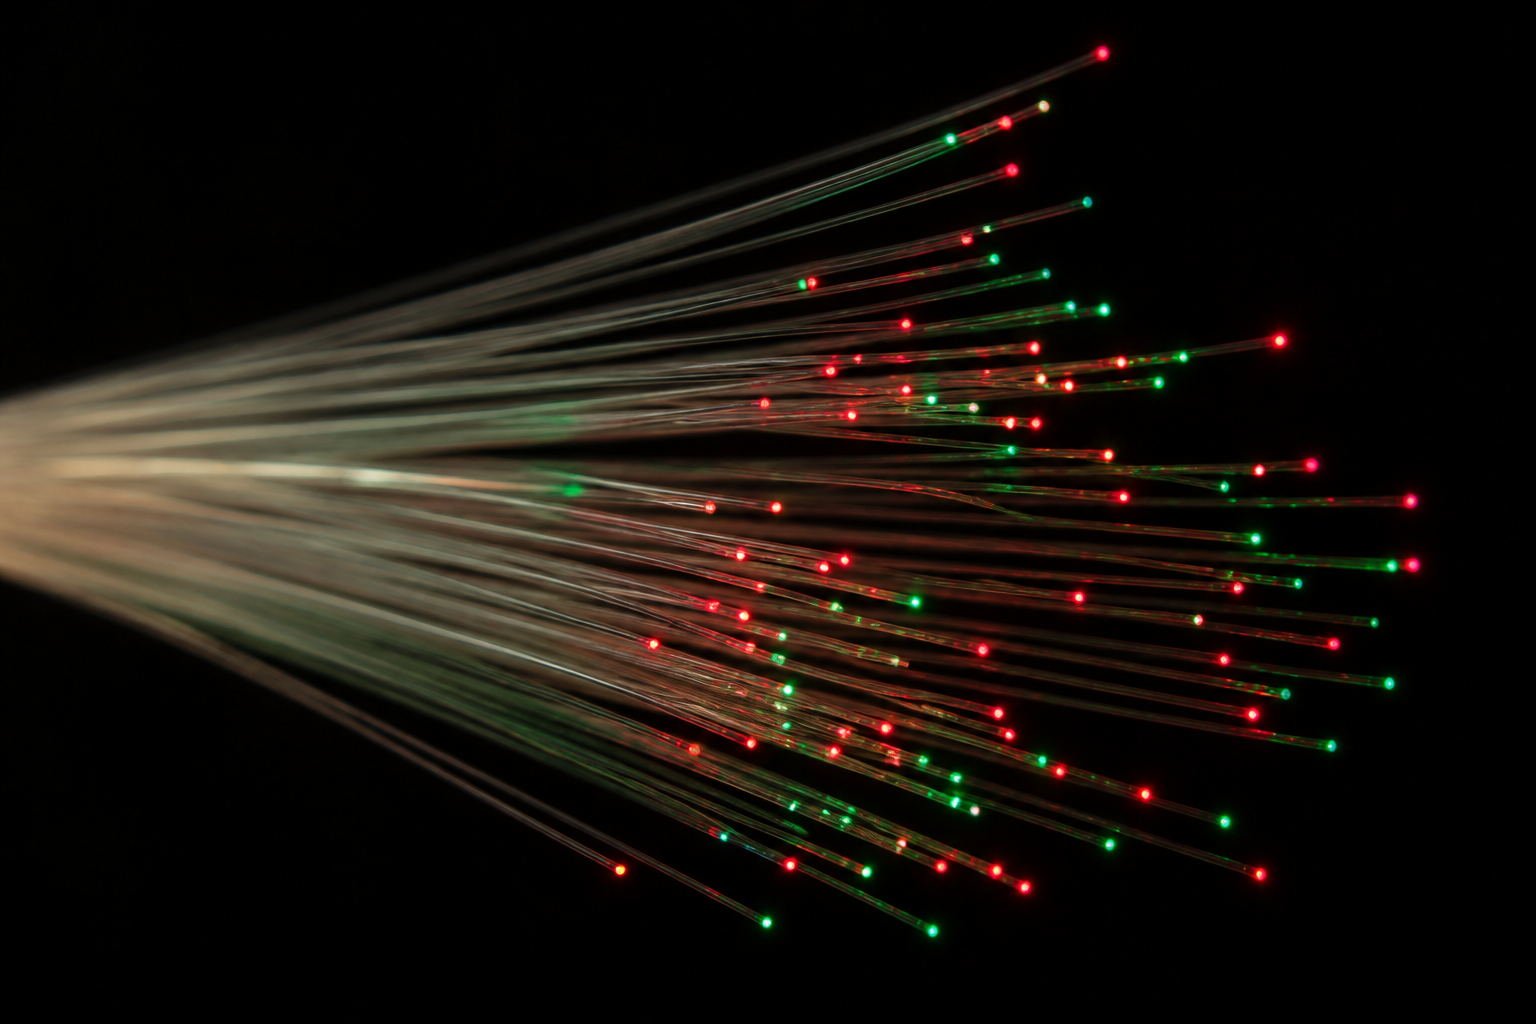
\includegraphics[width=0.58\linewidth]{images/book4/ai/b4-16-optical-fibres-glow.png}

{\small \omterm{prop:b2:guided-waves:fibre}{Fibras ópticas} iluminadas pelas pontas distantes: luz aprisionada por \omterm{thm:b2:wave-interfaces:snell}{reflexão total interna} num núcleo mais fino que um cabelo, e guiada em torno de cada curva suave.}
\end{omfigure}

\section{Problema: A cavidade do forno e a fibra óptica}

\begin{problem}[{Problema de fim de semana --- dois sistemas de ondas guiadas presentes em toda
cozinha e em toda cidade: o forno que cozinha com ondas estacionárias e
a fibra que carrega a internet}]
\label{pb:b2:guided-waves:1}

\medskip
\noindent\textbf{Parte I --- Do magnetron à cavidade.}
Um magnetron injeta \qty{800}{W} a \qty{2.45}{GHz} num \omterm{prop:b2:guided-waves:rectangular}{guia de ondas
retangular} ($a = \qty{8.6}{cm}$, $b = \qty{4.3}{cm}$) que desemboca na cavidade
do forno ($30 \times 30 \times 20$ cm$^3$); paredes de aço, $\gamma = \qty{1e6}{S/m}$.
\begin{enumerate}
  \item Frequências de corte dos \omterm{prop:b2:guided-waves:rectangular}{modos TE}$_{10}$, TE$_{20}$ e TE$_{01}$ do guia;
        verifique que só TE$_{10}$ se propaga a \qty{2.45}{GHz}.
  \item Comprimento de onda no guia e \omterm{def:b2:dispersion-wave-packets:relation}{velocidades de fase} e de grupo a \qty{2.45}{GHz}.
  \item Amplitude do campo $E_0$ no guia para \qty{800}{W} (fórmula da potência
        do TE$_{10}$); compare com o campo de ruptura do ar.
  \item Amplitude da \omterm{prop:b2:maxwell-equations:boundary}{corrente superficial} na parede larga (da ordem de
        $E_0/\mu_0c$); \omterm{def:b2:dispersion-wave-packets:complex}{profundidade de penetração} e resistência superficial do aço;
        perda por metro de guia.
  \item Modos da cavidade: liste os que têm frequência dentro de $3\%$
        de \qty{2.45}{GHz} (tente $(m, n, p)$ até $4$); quantos são?
  \item Distância entre os pontos quentes de um desses modos em cada
        eixo; por que o prato gira, e o que é um "agitador de modos"?
  \item O fator de qualidade da cavidade carregada com alimento vale cerca de
        $200$: largura de banda de sua resposta; por que um descasamento entre a
        frequência do magnetron e os modos não importa muito.
  \item A cavidade vazia tem $Q \approx 3000$: energia armazenada com \qty{800}{W}
        de entrada, densidade média de energia, amplitude do campo; compare com a
        questão 3 e com a ruptura. O que protege o magnetron
        quando o forno funciona vazio?
  \item Tempo que a energia leva para percorrer os \qty{20}{cm} de guia do
        magnetron até a cavidade.
  \item O magnetron é alimentado por uma fonte retificada de meia onda e só emite
        durante metade de cada ciclo da rede: potência de pico durante os
        surtos para uma média de \qty{800}{W}; o que a cavidade faz
        entre os surtos (use $Q \approx 200$)?
\end{enumerate}

\medskip
\noindent\textbf{Parte II --- A porta e o corte.}
\begin{enumerate}[resume]
  \item A tela da porta tem furos de \qty{1.5}{mm} numa chapa de \qty{1}{mm}: comprimento
        de decaimento num furo e \omterm{def:b2:dispersion-wave-packets:complex}{atenuação} em dB ao atravessar a chapa.
  \item A borda da porta é vedada por uma armadilha de quarto de onda: uma fenda
        de $\lambda/4$ de profundidade em volta do batente, que apresenta um circuito
        aberto na fresta (lembre o \cref{ch:b2:wave-interfaces}): profundidade
        da fenda a \qty{2.45}{GHz}.
  \item A fuga legal é de \qty{5}{mW/cm^2} a \qty{5}{cm}: a que fração de
        \qty{800}{W} através de uma porta de \qty{100}{cm^2} isso corresponde?
  \item Um duto de \qty{30}{cm} e \qty{4}{cm} de diâmetro ventila a cavidade: ele está
        abaixo do corte a \qty{2.45}{GHz}? \omterm{def:b2:dispersion-wave-packets:complex}{Atenuação} ao longo de seu comprimento.
  \item Por que a tela deve estar eletricamente unida ao batente da porta em todo o
        contorno (a que se pareceria uma falha nessa união)?
\end{enumerate}

\medskip
\noindent\textbf{Parte III --- A fibra.}
Uma fibra de índice degrau: núcleo $n_1 = 1.465$, casca $n_2 = 1.460$, diâmetro
do núcleo \qty{50}{\micro m} (multimodo) ou \qty{9}{\micro m} (monomodo);
$\lambda = \qty{1.55}{\micro m}$; \omterm{def:b2:dispersion-wave-packets:complex}{atenuação} de \qty{0.2}{dB/km}.
\begin{enumerate}[resume]
  \item \omterm{prop:b2:guided-waves:fibre}{Abertura numérica} e ângulo de aceitação; é fácil acoplar
        luz nela?
  \item Alargamento modal por quilômetro para a fibra multimodo; taxa máxima
        de bits em \qty{10}{km} (um bit por tempo de alargamento).
  \item Número de modos da fibra multimodo (admita $N \approx
        \tfrac12(\pi d\,\mathrm{NA}/\lambda)^2$); e da monomodo ($d =
        \qty{9}{\micro m}$: mostre que a mesma fórmula dá cerca de $1$).
  \item Na fibra monomodo o alargamento que resta é cromático:
        com $\omega'' \approx \qty{-0.2}{m^2/s}$ (\cref{ch:b2:dispersion-wave-packets})
        e pulsos de \qty{50}{ps}, distância em que um pulso dobra de largura;
        taxa de bits em \qty{100}{km}.
  \item \omterm{def:b2:dispersion-wave-packets:complex}{Atenuação} em \qty{100}{km}, em dB e como razão de potências; com
        \qty{1}{mW} de entrada: potência de saída; com amplificadores a cada \qty{80}{km},
        quantos são necessários para um enlace transatlântico de \qty{6000}{km}?
  \item Frequência e energia do fóton a \qty{1.55}{\micro m}; fótons por
        segundo em \qty{1}{mW}, e por bit a \qty{10}{Gbit/s}, na entrada
        e depois de \qty{100}{km}.
  \item Por que \qty{1.55}{\micro m} (pense nos dois mecanismos de perda da
        sílica: o espalhamento Rayleigh, que cai como $1/\lambda^4$, e a absorção
        no infravermelho, que cresce além de \qty{1.6}{\micro m})?
  \item Reflexão de Fresnel numa ponta de fibra clivada voltada para o ar: perda em
        dB; por que os conectores usam gel de casamento de índice ou contato
        físico polido.
  \item Por que uma fibra não irradia numa curva suave, e por que
        ela perde luz numa curva fechada (pense no ângulo do raio
        na fronteira do núcleo)?
  \item Compare os dois guias deste problema: o que confina a
        onda, o que limita a banda e quais são as perdas.
\end{enumerate}
\end{problem}
